\documentclass[../cnd.tex]{subfiles}

Ở chuỗi khối có những tính năng rất đặc biệt đó là có thể truyền tải dữ liệu mà không thông qua trung gian để xác nhận thông tin. Hệ thống chuỗi khối tồn tại nhiều nút độc lập với khả năng xác nhận thông tin. Mọi thông tin trong chuỗi khối có thể thay đổi hoặc bổ sung thêm khi có sự chấp nhận của tất cả các nút trên hệ thống. Hệ thống này có độ bảo mật cực cao mọi hành động đánh cắp dữ liệu đều sẽ bị chặn đứng. 

Chuỗi khối thậm chí vẫn hoạt động bình thường khi một phần của hệ thống sụp đổ, những máy tính và các nút vẫn hoạt động để bảo vệ thông tin, giữ cho chuỗi khối không bị mất dữ liệu.

\begin{figure}[H]
	\centering
	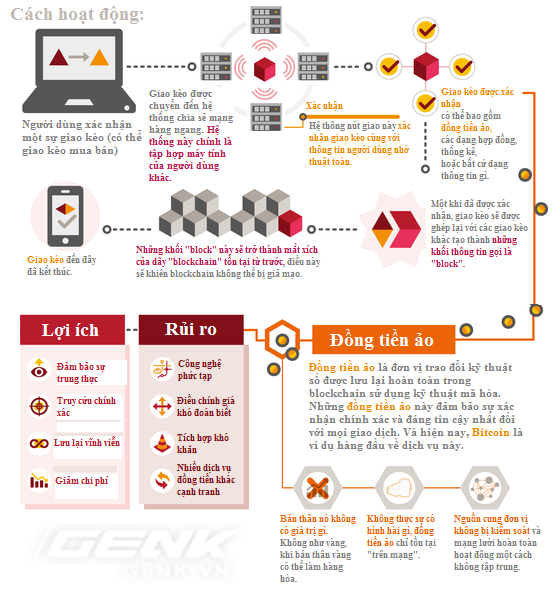
\includegraphics[width=0.8\linewidth]{../img/howtowork}
	\caption{Minh hoạ cách hoạt động của chuỗi khối$^{[5]}$}
	\label{fig:howtowork}
\end{figure}
